\section{Experimental Evaluation}

Using metadata-intesnvie and data-intensive benchmarks,
we evaluate our middleware's overall performance
and explore how its system design contribute to meeting its goals.
We specifically examine: (1) its improvement on the scability and
efficiency of metadata service for cluster file systems,
esepcially in concurrent file creation workloads;
(2) the data throughput in N-N checkpointing workloads
when layering our middleware on top of PanFS.

\textbf{Implementation }
Our middlware prototype is implemented in 14K lines of C using a modular desgin.
\tfs, \ldb and PanFS are modular plugins that can be replaced by other backends
that follow the API semantics. The current version implements most posix
file system operations except \texttt{hardlink}, \texttt{rename},
and operations for extended attributes.

\textbf{Evaluation System }
We evaluate the overall performance of our prototype
on two clusters with different settings.
One cluster is used to evaluate the scalability of \tfs and its integration with \giga.
The other cluster is used to evaluate the performance of layering our
prototype on top of a existing PanFS deployment.
The following table shows the detailed hardware and software configurations:

\begin{center}
\begin{tabular}{lcc}
\toprule
      & Cluster 1 & Cluster 2 \\
\midrule
\#Nodes & 64  &  5 \\
\hline
OS & Ubuntu 12.10  &   CentOS 6.3  \\
Kernel & 3.6.6 x86\_64 & 2.6.32 x86\_64\\
\hline
CPU & AMD Opteron 242   &  AMD Opteron 6272 \\
    & Dual Core & 6272 64 Cores\\
\hline
Memory & 16GB DDR &  128GB DDR \\
\hline
Network &       &           \\
\hline
Storage & Western Digital &  PanFS\\
System & Local hard disk &      5 Shelves \\
       &  2TB per node &   5MDS + 50 ODS \\
& 100 seeks/sec & \\
& rand. seeks        & \\
& 137.6 MB/sec & \\
& seq. reads      & \\
& 135.4 MB/sec & \\
& seq. writes      & \\
\bottomrule
\end{tabular}
\end{center}

In the following sections, we first evaluate each individual component
of our middlware, and finally evaluate end-to-end performance of
the integrated system on top of PanFS.

\subsection{Single Node Performance}

\subsection{Scalability Test on GIGA+TableFS}
Next, we evaluated the scalability of our distributed metadata middleware
prototype.
Figure \ref{graph:ldb-scaling} shows the instantaneous throughput during the
\textit{concurrent create} workload in a strong scaling experiment, i.e.
creating 1 million files per server, for a total of 64 million files in the
64-server configuration.
The main result in this figure is that as the number of servers doubles the
throughput of the system also scales up. With 64 servers, \giga{} can achieve a
peak throughput of about 190,000 file creates per second. The prototype delivers
peak performance after the directory workload has been spread among all
servers.
Reaching steady-state, the throughput quickly grows due to the splitting
policies adopted by \giga{}.

After reaching the steady state, throughput slowly drops as \ldb builds a
larger metadata store.
%Another observation in Figure \ref{graph:ldb-scaling} is that the system is
%unable to sustain the steady-state peak throughput (similar to our observation
%in the single-node test in Figure \ref{graph:ldb-singlenode}):
In fact, in large setups with 8 or more servers,
the peak throughput drops by as much as 25\% (in case of the 64-server setup).
This is because when there are more entries already existing in \ldb,
it requires more compaction work to maintain \ldb invariants and to perform a
negative lookup before each create has to search more SSTables on disk.
In theory, the work of inserting a new entry to a LSM-tree is $O(\log_{B}(n))$
where $n$ is the total number of inserted entries, and $B$ is a constant factor
proportional to the average number of entries transferred in each disk request
\cite{Bender2007}.
Thus we can use the formula $\frac{a\cdot S+b}{\log{T}}$ to
approximate the throughput timeline in Figure \ref{graph:ldb-scaling},
where $S$ is the number of servers, $T$ is the running time, and $a$ as well as $b$
are constant factors relative to the disk speed and splitting overhead.
This estimation projects that when inserting 64 billion files with 64 servers,
the system may deliver an average of 1,000 operations per second per server,
i.e. 64,000 operations per second in aggregate.

\begin{figure*}[t]  %%%%%%%%%%%%%%%%%%%%%%%
\centerline{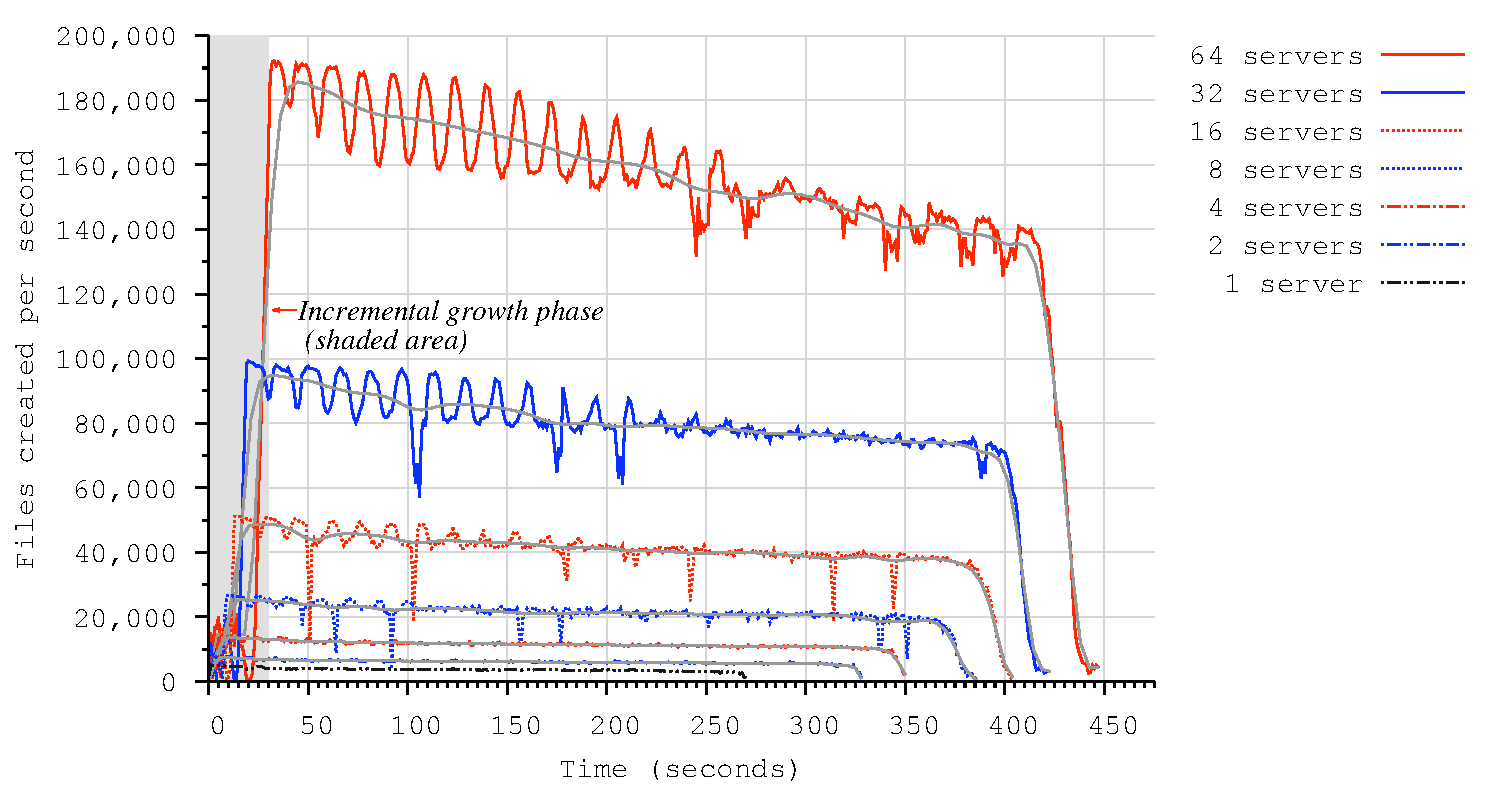
\includegraphics[scale=0.6]{./figs/ldb_insertrate}}
\vspace{10pt}
\caption{\normalsize
\textit{Our middleware metadata service prototype shows promising scalability
up to 64 servers.
Note that at the end of the experiment,
the throughput drops to zero
because clients stop creating files as they finish 1 million files per client.
And the solid lines in each configuration are Bezier
curves to smooth the variability.}
}
\vspace{10pt}
\hrule
\label{graph:ldb-scaling}
\end{figure*}       %%%%%%%%%%%%%%%%%%%%%%%

\subsection{Data Path Performance}


\begin{figure}[t]  %%%%%%%%%%%%%%%%%%%%%%%
\centerline{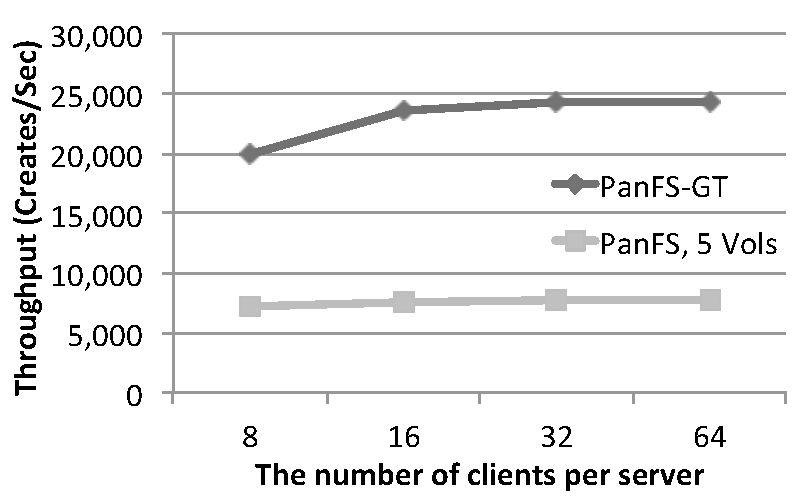
\includegraphics[scale=0.5]{./figs/zero_file_creation_on_panfs}}
\vspace{10pt}
\caption{\normalsize
Create five million zero-length files in one empty directory
with different number of clients.
\textit{}
}
\vspace{10pt}
\hrule
\label{graph:ldb-singlenode}
\end{figure}       %%%%%%%%%%%%%%%%%%%%%%%

\begin{figure}[t]  %%%%%%%%%%%%%%%%%%%%%%%
\centerline{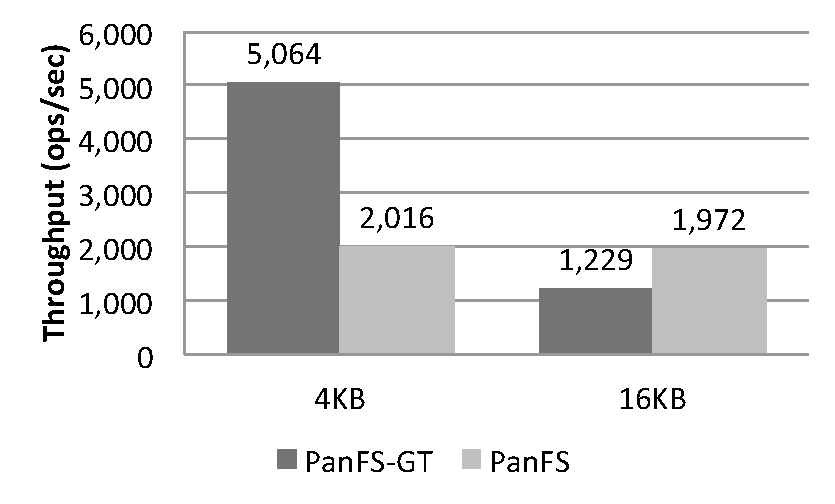
\includegraphics[scale=0.5]{./figs/small_file_creates}}
\vspace{10pt}
\caption{\normalsize
\textit{Create 5 million small files with different size
in one share directory}
}
\vspace{10pt}
\hrule
\label{graph:ldb-singlenode}
\end{figure}       %%%%%%%%%%%%%%%%%%%%%%%

\begin{figure}[t]  %%%%%%%%%%%%%%%%%%%%%%%
\centerline{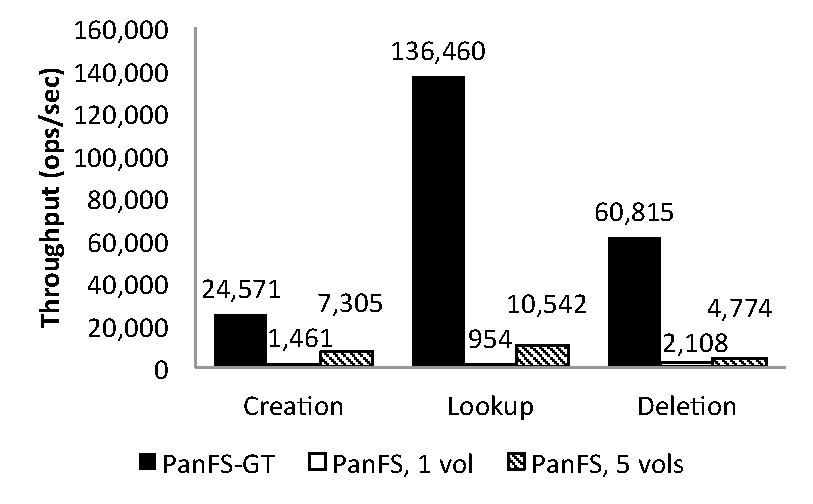
\includegraphics[scale=0.6]{./figs/mdtest}}
\vspace{10pt}
\caption{\normalsize
\textit{mdtest:
Create 5 million zero-length files in one shared directory.
}
}
\vspace{10pt}
\hrule
\label{graph:ldb-singlenode}
\end{figure}       %%%%%%%%%%%%%%%%%%%%%%%

\begin{figure}[t]  %%%%%%%%%%%%%%%%%%%%%%%
\centerline{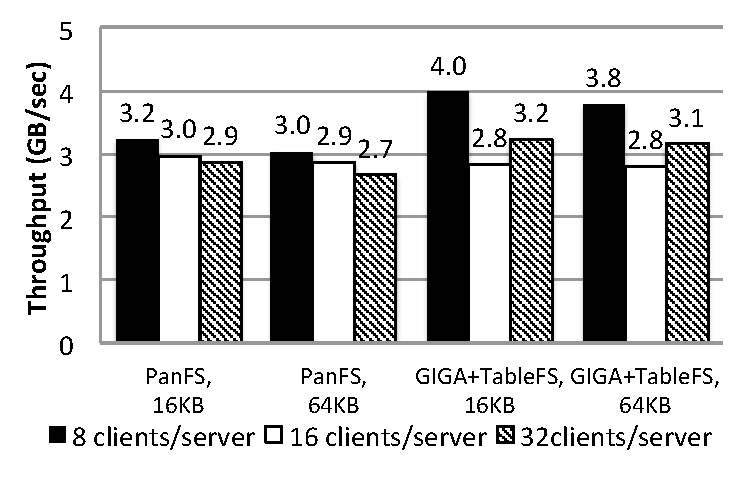
\includegraphics[scale=0.6]{./figs/checkpointing_write}}
\vspace{10pt}
\caption{\normalsize
\textit{
The aggregated write throughput in N-N check-pointing workload.
Each volume receives 640 GB data.
}
}
\vspace{10pt}
\hrule
\label{graph:ldb-singlenode}
\end{figure}       %%%%%%%%%%%%%%%%%%%%%%%

\begin{figure}[t]  %%%%%%%%%%%%%%%%%%%%%%%
\centerline{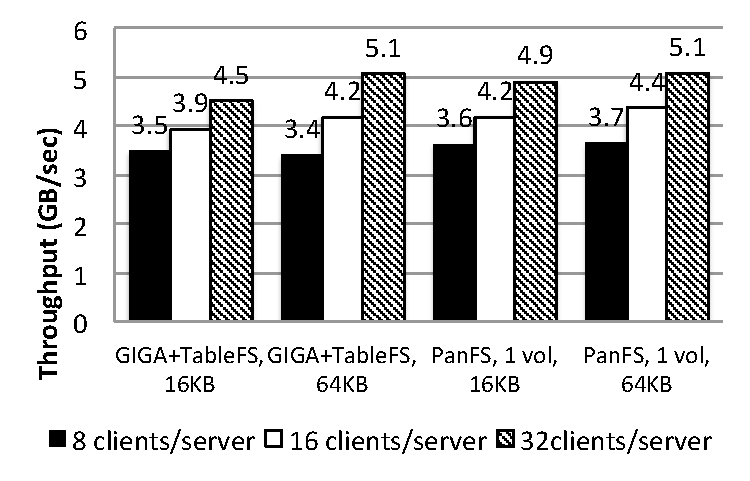
\includegraphics[scale=0.6]{./figs/checkpointing_read}}
\vspace{10pt}
\caption{\normalsize
\textit{
The aggregated read throughput in N-N check-pointing workload.
}
}
\vspace{10pt}
\hrule
\label{graph:ldb-singlenode}
\end{figure}       %%%%%%%%%%%%%%%%%%%%%%%

